% Important: If latex complains about unicode characters,
% please use "\usepackage[utf8x]{inputenc}" in your preamble
% You can change the size of the picture by putting it into the construct:
% 1) \resizebox{10cm}{!}{"below picture"} to scale horizontally to 10 cm
% 2) \resizebox{!}{15cm}{"below picture"} to scale vertically to 15 cm
% 3) \resizebox{10cm}{15cm}{"below picture"} a combination of above two
% It is not recomended to use the scale option of the tikzpicture environment.
\resizebox{7cm}{!}{
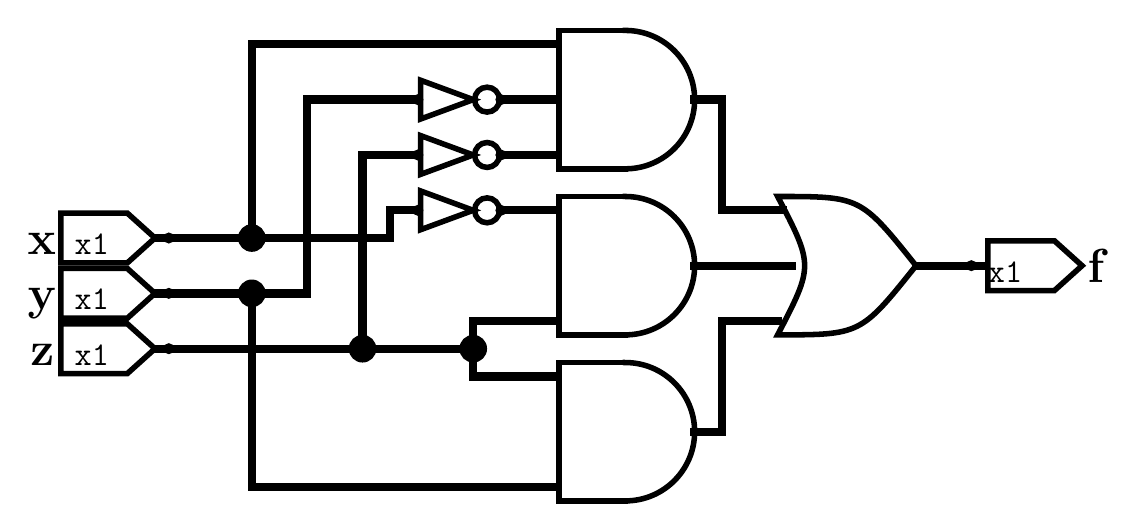
\begin{tikzpicture}[x=1pt,y=-1pt,line cap=rect]
\def\logisimfontA#1{\fontfamily{cmr}{#1}} % Replaced by logisim, original font was "SansSerif"
\def\logisimfontB#1{\fontfamily{cmtt}{#1}} % Replaced by logisim, original font was "Monospaced"
\definecolor{custcol_0_0_0}{RGB}{0, 0, 0}
\definecolor{custcol_ff_ff_ff}{RGB}{255, 255, 255}
\draw [line width=3.0pt, custcol_0_0_0 ]  (326.0,90.0) -- (346.0,90.0) ;
\draw [line width=3.0pt, custcol_0_0_0 ]  (196.0,10.0) -- (86.0,10.0) -- (86.0,80.0) -- (136.0,80.0) -- (136.0,70.0) -- (146.0,70.0) ;
\draw [line width=3.0pt, custcol_0_0_0 ]  (126.0,120.0) -- (166.0,120.0) ;
\draw [line width=3.0pt, custcol_0_0_0 ]  (196.0,110.0) -- (166.0,110.0) -- (166.0,120.0) -- (166.0,130.0) -- (196.0,130.0) ;
\draw [line width=3.0pt, custcol_0_0_0 ]  (176.0,50.0) -- (196.0,50.0) ;
\draw [line width=3.0pt, custcol_0_0_0 ]  (176.0,30.0) -- (196.0,30.0) ;
\draw [line width=3.0pt, custcol_0_0_0 ]  (176.0,70.0) -- (196.0,70.0) ;
\draw [line width=3.0pt, custcol_0_0_0 ]  (86.0,100.0) -- (106.0,100.0) -- (106.0,30.0) -- (146.0,30.0) ;
\fill [line width=3.0pt, custcol_0_0_0]  (166.0,120.0) ellipse (5.0 and 5.0 );
\fill [line width=3.0pt, custcol_0_0_0]  (126.0,120.0) ellipse (5.0 and 5.0 );
\fill [line width=3.0pt, custcol_0_0_0]  (86.0,80.0) ellipse (5.0 and 5.0 );
\fill [line width=3.0pt, custcol_0_0_0]  (86.0,100.0) ellipse (5.0 and 5.0 );
\draw [line width=3.0pt, custcol_0_0_0 ]  (350.0,90.0) -- (347.0,90.0) ;
\draw [line width=2.0pt, custcol_0_0_0 ]  (376.0,81.0) -- (386.0,90.0) -- (376.0,99.0) -- (352.0,99.0) -- (352.0,81.0) -- cycle;
\logisimfontB{\fontsize{12pt}{12pt}\selectfont\node[inner sep=0, outer sep=0, custcol_0_0_0, anchor=base west] at  (352.0,96.0)  {x1};}
\logisimfontA{\fontsize{16pt}{16pt}\fontseries{bx}\selectfont\node[inner sep=0, outer sep=0, custcol_0_0_0, anchor=base west] at  (388.0,96.0)  {f};}
\fill [line width=2.0pt, custcol_0_0_0]  (346.0,90.0) ellipse (2.0 and 2.0 );
\draw [line width=3.0pt, custcol_0_0_0 ]  (51.0,120.0) -- (56.0,120.0) -- (126.0,120.0) -- (126.0,50.0) -- (146.0,50.0) ;
\draw [line width=2.0pt, custcol_0_0_0 ]  (41.0,129.0) -- (51.0,120.0) -- (41.0,111.0) -- (17.0,111.0) -- (17.0,129.0) -- cycle;
\logisimfontB{\fontsize{12pt}{12pt}\selectfont\node[inner sep=0, outer sep=0, custcol_0_0_0, anchor=base west] at  (22.0,126.0)  {x1};}
\logisimfontA{\fontsize{16pt}{16pt}\fontseries{bx}\selectfont\node[inner sep=0, outer sep=0, custcol_0_0_0, anchor=base west] at  (6.0,126.0)  {z};}
\fill [line width=2.0pt, custcol_0_0_0]  (56.0,120.0) ellipse (2.0 and 2.0 );
\draw [line width=3.0pt, custcol_0_0_0 ]  (51.0,100.0) -- (56.0,100.0) -- (86.0,100.0) -- (86.0,170.0) -- (196.0,170.0) ;
\draw [line width=2.0pt, custcol_0_0_0 ]  (41.0,109.0) -- (51.0,100.0) -- (41.0,91.0) -- (17.0,91.0) -- (17.0,109.0) -- cycle;
\logisimfontB{\fontsize{12pt}{12pt}\selectfont\node[inner sep=0, outer sep=0, custcol_0_0_0, anchor=base west] at  (22.0,106.0)  {x1};}
\logisimfontA{\fontsize{16pt}{16pt}\fontseries{bx}\selectfont\node[inner sep=0, outer sep=0, custcol_0_0_0, anchor=base west] at  (5.0,106.0)  {y};}
\fill [line width=2.0pt, custcol_0_0_0]  (56.0,100.0) ellipse (2.0 and 2.0 );
\draw [line width=3.0pt, custcol_0_0_0 ]  (246.0,30.0) -- (256.0,30.0) -- (256.0,70.0) -- (276.0,70.0) -- (278.0,70.0) ;
\draw [line width=3.0pt, custcol_0_0_0 ]  (246.0,90.0) -- (276.0,90.0) -- (281.0,90.0) ;
\draw [line width=3.0pt, custcol_0_0_0 ]  (246.0,150.0) -- (256.0,150.0) -- (256.0,110.0) -- (276.0,110.0) -- (276.0,110.0) ;
\draw [line width=2.0pt, custcol_0_0_0 ]  (326.0,90.0) .. controls  (306.0,65.0)  ..  (276.0,65.0) .. controls  (289.0,90.0)  ..  (276.0,115.0) .. controls  (306.0,115.0)  ..  (326.0,90.0) -- cycle ;
\draw [line width=2.0pt, custcol_0_0_0 ]  (166.0,70.0) -- (147.0,63.0) -- (147.0,77.0) -- cycle;
\draw [line width=2.0pt, custcol_0_0_0]  (171.0,70.0) ellipse (4.5 and 4.5 );
\fill [line width=2.0pt, custcol_0_0_0]  (176.0,70.0) ellipse (2.0 and 2.0 );
\fill [line width=2.0pt, custcol_0_0_0]  (146.0,70.0) ellipse (2.0 and 2.0 );
\draw [line width=2.0pt, custcol_0_0_0] (221.0,115.0) arc (90.0:-90.0:25.0 and 25.0 );
\draw [line width=2.0pt, custcol_0_0_0 ]  (221.0,65.0) -- (197.0,65.0) -- (197.0,115.0) -- (221.0,115.0) ;
\draw [line width=2.0pt, custcol_0_0_0 ]  (166.0,30.0) -- (147.0,23.0) -- (147.0,37.0) -- cycle;
\draw [line width=2.0pt, custcol_0_0_0]  (171.0,30.0) ellipse (4.5 and 4.5 );
\fill [line width=2.0pt, custcol_0_0_0]  (176.0,30.0) ellipse (2.0 and 2.0 );
\fill [line width=2.0pt, custcol_0_0_0]  (146.0,30.0) ellipse (2.0 and 2.0 );
\draw [line width=2.0pt, custcol_0_0_0 ]  (166.0,50.0) -- (147.0,43.0) -- (147.0,57.0) -- cycle;
\draw [line width=2.0pt, custcol_0_0_0]  (171.0,50.0) ellipse (4.5 and 4.5 );
\fill [line width=2.0pt, custcol_0_0_0]  (176.0,50.0) ellipse (2.0 and 2.0 );
\fill [line width=2.0pt, custcol_0_0_0]  (146.0,50.0) ellipse (2.0 and 2.0 );
\draw [line width=3.0pt, custcol_0_0_0 ]  (51.0,80.0) -- (56.0,80.0) -- (86.0,80.0) ;
\draw [line width=2.0pt, custcol_0_0_0 ]  (41.0,89.0) -- (51.0,80.0) -- (41.0,71.0) -- (17.0,71.0) -- (17.0,89.0) -- cycle;
\logisimfontB{\fontsize{12pt}{12pt}\selectfont\node[inner sep=0, outer sep=0, custcol_0_0_0, anchor=base west] at  (22.0,86.0)  {x1};}
\logisimfontA{\fontsize{16pt}{16pt}\fontseries{bx}\selectfont\node[inner sep=0, outer sep=0, custcol_0_0_0, anchor=base west] at  (5.0,86.0)  {x};}
\fill [line width=2.0pt, custcol_0_0_0]  (56.0,80.0) ellipse (2.0 and 2.0 );
\draw [line width=2.0pt, custcol_0_0_0] (221.0,175.0) arc (90.0:-90.0:25.0 and 25.0 );
\draw [line width=2.0pt, custcol_0_0_0 ]  (221.0,125.0) -- (197.0,125.0) -- (197.0,175.0) -- (221.0,175.0) ;
\draw [line width=2.0pt, custcol_0_0_0] (221.0,55.0) arc (90.0:-90.0:25.0 and 25.0 );
\draw [line width=2.0pt, custcol_0_0_0 ]  (221.0,5.0) -- (197.0,5.0) -- (197.0,55.0) -- (221.0,55.0) ;
\end{tikzpicture}
}

